\label{Chapter2}

\section{Περιγραφή φυσικού αντικειμένου}

Το γενικό αντικείμενο της εργασίας είναι μία διακήρυξη διαγωνισμού από την Ηλεκτρονική Διακυβέρνηση Κοινωνικής Ασφάλισης (ΗΔΙΚΑ) που ονομάζεται <<Ενιαίο Πληροφοριακό Σύστημα για την Υποστήριξη των Επιχειρησιακών Λειτουργικών Μονάδων Υγείας του ΕΣΥ>>. Ο γενικός προϋπολογισμός με ΦΠΑ είναι 17.250.000\euro, ενώ χωρίς ΦΠΑ 14.024.390,24\euro. Στην ομάδα έχει αναθέτει το υποσύστημα Α.4.3.7 <<Διαχείριση Αποθηκών>>. Θα γίνει ανάλυση του υποσυστήματος μέσω του διαγράμματος WBS και θα γίνει ο απαραίτητος χρονικός προγραμματισμός με την χρήση του Gantt, τον προγραμματισμό των πόρων και τον προϋπολογισμό.

\subsection{Διαχείριση αποθηκών}

Η διαχείριση των αποθηκών είναι ένα υποσύστημα της πλατφόρμας που θα δημιουργηθεί, το οποίο είναι υπεύθυνο για τον έγκαιρο προγραμματισμό του εφοδιασμού της Μονάδας Υγείας με υλικά και η αποτελεσματική εξυπηρέτηση της με ταυτόχρονη ελαχιστοποίηση. Θα είναι επίσης υπεύθυνο να γίνει σωστή αντιστοιχίσει των παραμέτρων που θα δέχεται με όλους τους τύπους που μπορεί να δεχθεί.

\begin{problem}
  ``Η εφαρμογή της Διαχείρισης Αποθηκών χρησιμοποιείται για την παρακολούθηση και τον έλεγχο των
  υλικών και των αποθηκών της Μονάδας Υγείας. Απεικονίζει και παρακολουθεί όλες τις Αποθήκες, τους
  Αποθηκευτικούς Χώρους και τις θέσεις Αποθήκευσης. \par

  Οι αποθήκες ενημερώνονται άμεσα από τις παραλαβές των προμηθειών, από τις διακινήσεις μεταξύ
  αποθηκών και τις αναλώσεις ενώ τηρείται ανά πάσα στιγμή ενημερωμένο υπόλοιπο ανά είδος και
  αποθήκη''

  Επίσημο έγγραφο από ΗΔΙΚΑ για την διακήρυξη του διαγωνισμού
\end{problem}

\subsubsection{Οι λειτουργίες της εφαρμογής}
\label{chap:workflow}

Οι βασικές λειτουργίες της εφαρμογής είναι:

\begin{enumerate}
  \item \textbf{Οργάνωση αποθηκών}: να υπάρχει η δυνατότητα συντήρησης και απεικόνισης πολλαπλών αποθηκών και διακριτών αποθηκευτικών χώρων.
  \item \textbf{Αρχείο ειδών}: να υπάρχει ένα αρχείο το οποίο θα κρατάει πληροφορίες σχετικά με τα αποθηκεύσιμα είδη το οποίο θα είναι κοινό για όλες τις αποθήκες και τα τμήματα. Μερικές πληροφορίες που θα μπορούσε να κρατάει είναι:
    \begin{itemize}
      \item Βασικά στοιχεία υλικού (κωδικός, συνοπτική και αναλυτική περιγραφή υλικού)
      \item Μονάδες μέτρησης
      \item Ομάδες Υλικών:
        \begin{itemize}
          \item Ομαδοποίηση βάσει της φύσης του υλικού.
          \item Ιεραρχία ειδών.
          \item Κατηγορίες υλικών και χαρακτηριστικά.
        \end{itemize}
      \item Επίπεδο αναπαραγγελίας και απόθεμα ασφάλειας.
    \end{itemize}
  \item \textbf{Διαχείριση αλλαγών}: η δυνατότητα πρόσβασης στο αρχείο υλικών και η δυνατότητα αλλαγής των στοιχείων αυτού από εξουσιοδοτημένους χρήστες.
  \item \textbf{Διαχείριση παρτίδων}: Η παρτίδα θα χαρακτηρίζεται από την ημερομηνία λήξης, ενώ θα υπάρχει η δυνατότητα δημιουργίας χαρακτηριστικών οριζόμενων από τον χρήστη, τα οποία ενημερώνονται κατά την δημιουργία της και έχουν σαν σκοπό την καταγραφή των ποιοτικών και άλλων χαρακτηριστικών. Η διαχείριση και η παραλαβή των πατρίδων θα πρέπει να ακολουθάνε μερικούς κανόνες:
    \begin{itemize}
      \item Κατά την παραλαβή στην αποθήκη θα πρέπει να απαιτείται καταχώρηση της ημερομηνίας λήξης.
      \item Κατά την εξαγωγή θα πρέπει να υπάρχει η δυνατότητα αυτόματης επιλογής.
    \end{itemize}
  \item \textbf{Ψηφιακοί κωδικοί (Barcodes)}
  \item \textbf{Κινήσεις αποθήκης}: Όλες οι εισαγωγές, οι εξαγωγές και οι διακινήσεις θα πρέπει να αποτυπώνονται στην αποθήκη με κωδικούς και με αιτίες. Κάθε κίνηση αποθήκης συνοδεύεται από μία αντίστροφη/ακυρωτική κίνηση, η οποία εκτελείται σε περίπτωση ακύρωσης και η οποία έχει αντίθετο αποτέλεσμα. Συγκεκριμένα, οι κινήσεις είναι οι εξής:
    \begin{itemize}
      \item Εισαγωγές: στις εισαγωγές θα πρέπει να περιλαμβάνεται κυρίως η παραλαβή από αγορά. Θα πρέπει να δίνετε δυνατότητα εύκολης ανεύρεσης των ανοιχτών εντολών αγοράς, βάσει κριτηρίων. Κατά την παραλαβή, ενημερώνεται αυτόματα η αποθήκη και τα ιστορικά στοιχεία προμηθειών.
      \item Εξαγωγές: Εξαγωγές από την αποθήκη είναι όλες οι αναλώσεις υλικών, οι επιστροφές σε προμηθευτές κλπ.
      \item Ενδοδιακινήσεις: Θα υποστηρίζονται ενδοδιακινήσεις αποθέματος από την κεντρική αποθήκη προς τα τμήματα καθώς και μεταξύ τμημάτων ή μονάδων υγείας.
      \item Λοιπές κινήσεις: Εκτός από τις ανωτέρω κινήσεις, θα υποστηρίζονται και λοιπές κινήσεις όπως είναι, καταστροφή, διαφορές απογραφής, τακτοποιήσεις αποθέματος κλπ
    \end{itemize}
  \item \textbf{Φυσική απογραφή - Προσαρμογές αποθήκης}: Φυσική καταμέτρηση των είδων μπορεί να γίνεται είτε περιοδικά μέσα στο έτος είτε στο τέλος αυτού. Η διαδικασία περιλαμβάνει τα εξής:
    \begin{itemize}
      \item Επιλογή των αποθηκών στις οποίες πρόκειται να γίνει φυσική απογραφή
      \item Δημιουργία βοηθητικών φύλλων καταγραφής των υλικών της αποθήκης
      \item Κλείδωμα των προς καταμέτρηση αποθηκών για αποφυγή κινήσεων κατά την διάρκεια της απογραφής
      \item Καταχώρηση των αποτελεσμάτων της καταμέτρησης (το σύστημα ενημερώνει για τυχόν διαφορές του πραγματικού με το λογιστικό υπόλοιπο)
      \item Δυνατότητα επανακαταμέτρησης για όσα είδη επιλέξει ο χρήστης
      \item Αυτόματη καταχώρηση διορθωτικών κινήσεων στην περίπτωση αποδοχής των διαφορών από εξουσιοδοτημένους χρήστες
    \end{itemize}
  \item \textbf{Άλλα χαρακτηριστικά} όπως:
    \begin{itemize}
      \item \textbf{Αποτίμηση Υλικών}
      \item \textbf{Βιβλίο Αποθήκης}
      \item \textbf{Αναφορές - Καταστάσεις}
        \begin{itemize}
          \item Συγκεντρωτική και αναλυτική αναφορά
          \item Επισκόπηση αποθέματος
          \item Δυνατότητα άμεσης παρακολούθησης των κινήσεων εισαγωγών
          \item Αναφορές αποτίμησης αποθήκης
          \item Αναφορά όλων των υλικών με μηδενικό απόθεμα ή απόθεμα κάτω από το όριο ασφάλειας
        \end{itemize}
    \end{itemize}
\end{enumerate}

Το υποσύστημα της διαχείρισης αποθηκών διασυνδέεται με τα υπόλοιπα συστήματα όπως παρουσιάζεται στο Σχήμα~\ref{fig:subsystems}.

\begin{figure}[H]
  \centering
  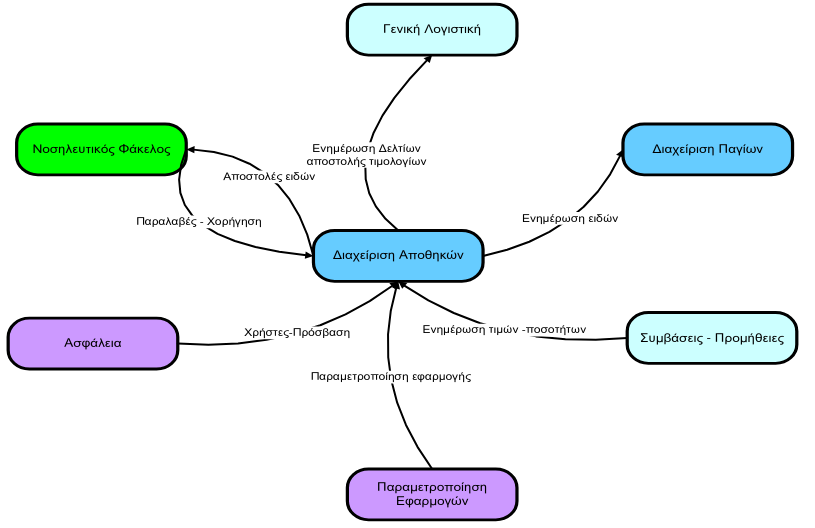
\includegraphics[width=150mm]{Figures/subsystems.png}
  \caption[Οι σχέσεις της Διαχείρισης Αποθηκών με τα υπόλοιπα υποσυστήματα]{Η διασύνδεση του υποσυστήματος της Διαχείρισης Αποθηκών με τα υπόλοιπα υποσυστήματα}
  \label{fig:subsystems}
\end{figure}

\subsubsection{Αναπαράσταση δομής σε διαγράμμα WBS}

Ένα διάγραμμα \textbf{Work Breakdown Structure (WBS)} είναι μία εικονική, ιεραρχική και παραδοτέα αναπαράσταση ενός project. Υπάρχουν τρία είδη των WBS διαγραμμάτων.

\begin{itemize}
  \item Το \textbf{WBS List} το οποίο παρουσιάζει σε λίστες τα διάφορα πακέτα από δουλεία, εργασιών και παραδοτέων που πρέπει να ετοιμαστούν.
  \item Το \textbf{WBS Tree Diagram} το οποίο εμφανίζεται πιο συχνά από τα υπόλοιπα και παρουσιάζει την ροή των εργασιών και των φάσεων.
  \item Το \textbf{WBS Gantt Chart} το οποίο είναι ένα σχεδιάγραμμα από ένα spreadsheet και ένα timeline το οποίο παρουσιάζει τον χρονοπρογραμματισμό των φάσεων.
\end{itemize}

Με βάση το Κεφάλαιο~\ref{chap:workflow}, το σχεδιάγραμμα WBS List απεικονίζεται στο Σχήμα~\ref{fig:wbs_ver1}.

\begin{figure}[H]
  \centering
  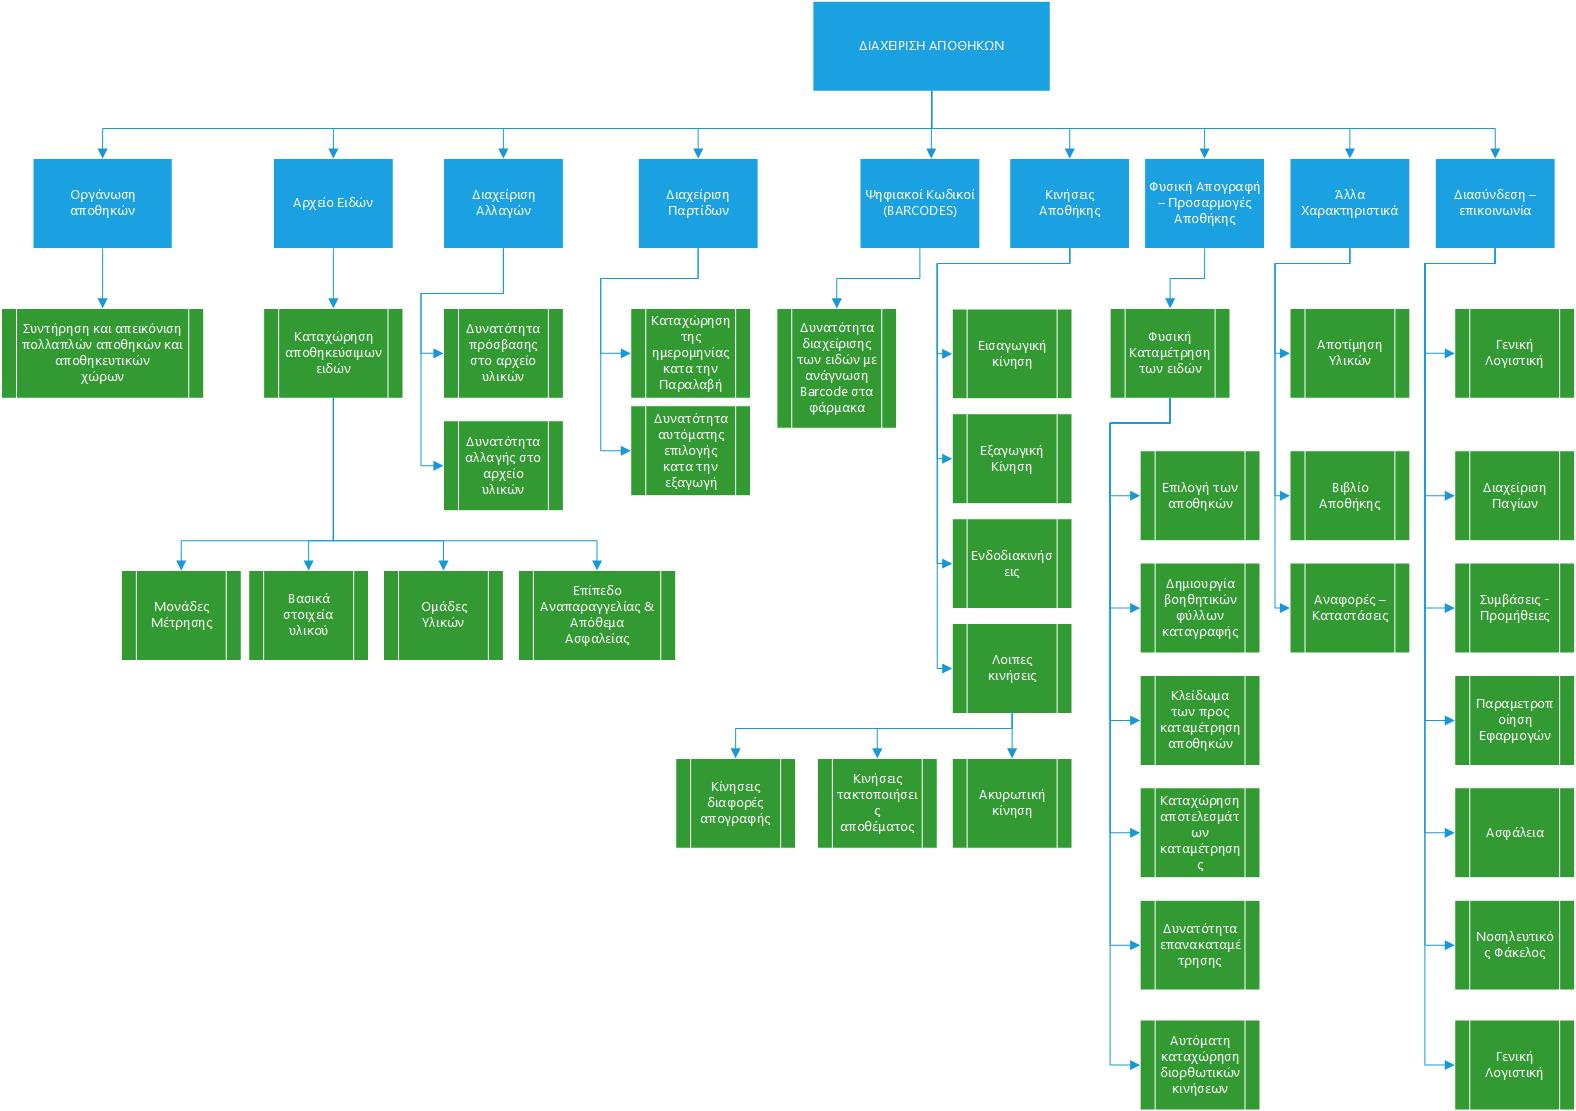
\includegraphics[width=150mm]{Figures/wbs_ver1.jpg}
  \caption{Αναπαράσταση δομής σε διάγραμμα WBS}
  \label{fig:wbs_ver1}
\end{figure}

\subsection{Εφαρμογή του SCRUM στην Διαχείριση Αποθηκών}

Σύμφωνα με το Κεφάλαιο~\ref{chap:scrum}, οι φάσεις της Διαχείρισης Αποθηκών πρέπει να είναι οι ακόλουθες:

\begin{itemize}
  \item Όραμα του project (δόθηκε έτοιμο από τον διαγωνισμό)
  \item Πλάνο κυκλοφορίας
  \item Πλάνο του Spring (τρέχον φάση) και τις φάσεις του
  \item Αρχή ενός Spring με την φάση της ανάλυσης
  \item Υλοποίηση του υποσυστήματος και παράλληλο scale up στο deployment της εφαρμογής
  \item Καθημερινό meeting για να συζητηθεί η πορεία της ομάδας και να γίνει αξιολόγηση της δουλείας
  \item Εύρεση λαθών και επανάληψης του Spring για να διορθωθούν λάθη ή να γίνει υλοποίηση νέων λειτουργιών
\end{itemize}

\subsubsection{Αναπαράσταση φάσεων σε διάγραμμα WBS}

\subsubsection{Αναπαράσταση χρονοπρογραμματισμού σε διάγραμμα WBS}

\subsection{Προγραμματισμός πόρων και τελικός προϋπολογισμός}
